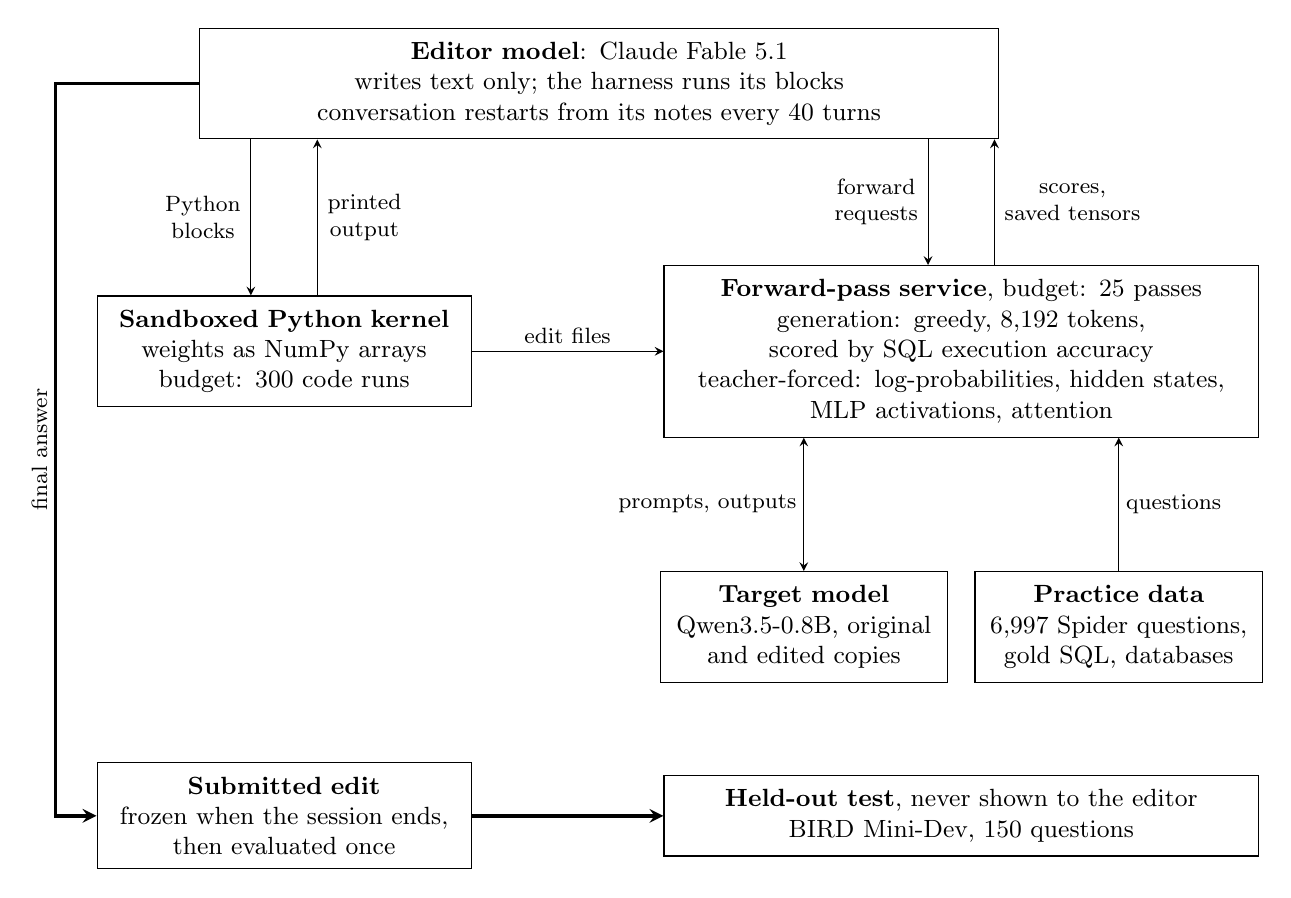
\begin{tikzpicture}[font=\small, box/.style={draw, align=center, inner sep=5pt, text width=#1}, box/.default=4.4cm, lab/.style={font=\footnotesize, fill=white, inner sep=1.5pt, align=center}, >=stealth]
\node[box=9.8cm] (E) at (4.6,0) {\textbf{Editor model}: Claude Fable 5.1\\writes text only; the harness runs its blocks\\conversation restarts from its notes every 40 turns};
\node[box=4.4cm] (K) at (0.6,-3.4) {\textbf{Sandboxed Python kernel}\\weights as NumPy arrays\\budget: 300 code runs};
\node[box=7.2cm] (F) at (9.2,-3.4) {\textbf{Forward-pass service}, budget: 25 passes\\generation: greedy, 8,192 tokens,\\scored by SQL execution accuracy\\teacher-forced: log-probabilities, hidden states,\\MLP activations, attention};
\node[box=3.3cm] (M) at (7.2,-6.9) {\textbf{Target model}\\Qwen3.5-0.8B, original\\and edited copies};
\node[box=3.3cm] (P) at (11.2,-6.9) {\textbf{Practice data}\\6,997 Spider questions,\\gold SQL, databases};
\node[box=4.4cm] (S) at (0.6,-9.3) {\textbf{Submitted edit}\\frozen when the session ends,\\then evaluated once};
\node[box=7.2cm] (H) at (9.2,-9.3) {\textbf{Held-out test}, never shown to the editor\\BIRD Mini-Dev, 150 questions};
\draw[->] ([xshift=-12pt]E.south west -| K.north) -- node[lab, left=2pt] {Python\\blocks} ([xshift=-12pt]K.north);
\draw[<-] ([xshift=12pt]E.south west -| K.north) -- node[lab, right=2pt] {printed\\output} ([xshift=12pt]K.north);
\draw[->] ([xshift=-12pt]E.south -| F.north) -- node[lab, left=2pt] {forward\\requests} ([xshift=-12pt]F.north);
\draw[<-] ([xshift=12pt]E.south -| F.north) -- node[lab, right=2pt] {scores,\\saved tensors} ([xshift=12pt]F.north);
\draw[->] (K) -- node[lab, above=1pt] {edit files} (F);
\draw[<->] (M.north) -- node[lab, left=1pt] {prompts, outputs} (M.north |- F.south);
\draw[->] (P.north) -- node[lab, right=1pt] {questions} (P.north |- F.south);
\draw[->, very thick] (E.west) -- (-2.3,0) -- node[lab, rotate=90, above=1pt] {final answer} (-2.3,-9.3) -- (S.west);
\draw[->, very thick] (S) -- (H);
\end{tikzpicture}
